\documentclass[11pt]{article}

\usepackage{extras} % Se extras.sty

\begin{document}
\begin{titlepage}
\begin{center}

{\Large\bfseries TSEA56 - Kandidatprojekt i elektronik \\ LIPS Kappa}

\vspace{5em}

Version 1.0

\vspace{5em}
Grupp 4 \\
\begin{tabular}{rl}
Hynén Ulfsjöö, Olle&\verb+ollul666+
\\
Wasteson, Emil&\verb+emiwa068+
\\
Tronje, Elena&\verb+eletr654+
\\
Gustafsson, Lovisa&\verb+lovgu777+
\\
Inge, Zimon&\verb+zimin415+
\\
Strömberg, Isak&\verb+isast763+
\\
\end{tabular}

\vspace{5em}
\today

\vspace{16em}
Status
\begin{longtable}{|l|l|l|} \hline

Granskad & - & - \\ \hline
Godkänd & - & - \\ \hline
 
\end{longtable}

\end{center}
\end{titlepage}

\pagebreak
\begin{center}

\section*{PROJEKTIDENTITET}
2016/VT, Undsättningsrobot Gr. 4

Linköpings tekniska högskola, ISY
\vspace{5em}
%\begin{center}

\begin{tabular}{|l|l|l|l|} \hline
\textbf{Namn} & \textbf{Ansvar} & \textbf{Telefon} & \textbf{E-post}  \\ \hline 
Isak Strömberg (IS) & Projektledare & 073-980 38 50 & isast763@student.liu.se \\ \hline
Olle Hynén Ulfsjöö (OHU)& Dokumentansvarig & 070-072 91 84 & ollul666@student.liu.se \\ \hline
Emil Wasteson (EW) & Hårdvaruansvarig & 076-836 61 66 & emiwa068@student.liu.se \\ \hline
Elena Tronje (ET) & Mjukvaruansvarig & 072-276 92 93 & eletr654@student.liu.se \\ \hline
Zimon Inge (ZI)& Testansvarig & 070-171 35 18 & zimin415@student.liu.se \\ \hline
Lovisa Gustafsson (LG) & Leveransansvarig & 070-210 32 53 & lovgu777@student.liu.se \\ \hline
\end{tabular}

%\end{center}

E-postlista för hela gruppen: isast763@student.liu.se

\vspace{5em}
Kund: ISY, Linköpings universitet 
tel: 013-28 10 00, fax: 013-13 92 82 \\
Kontaktperson hos kund: Mattias Krysander \\
tel: 013-28 21 98, e-post: matkr@isy.liu.se \\

\vspace{5em}
Kursansvarig:  Tomas Svensson\\
tel: 013-28 13 68, e-post: tomass@isy.liu.se \\
Handledare: Peter Johansson \\
tel: 013-28 13 45, e-post: peter.a.johansson@liu.se
\end{center}
\pagebreak

\tableofcontents

\pagebreak

\section*{Dokumenthistorik}
\begin{table}[h]
\begin{tabular}{|l|l|l|l|l|} \hline

\textbf{Version} & \textbf{Datum} & \textbf{Utförda förändringar} & \textbf{Utförda av} & \textbf{Granskad} \\ \hline
1.0 & - &  Första utkastet & Grupp 4 & - \\ \hline
\end{tabular}
\end{table}

\pagebreak
\pagenumbering{arabic}

\begin{flushleft}
\section{Inledning}
\textit{Ge en översiktlig beskrivning av produkten och uppdraget gärna kopplat till bilder.}
\textit{Lyft gärna fram det som ni anser är utmanande/intressant i uppdraget.}
\textit{Beskriv kortfattat dispositionen på rapporten.}


Uppdraget var att konstruera en autonom undsättningsrobot med kartläggning för utforskning av ett okänt grottsystem. I grottsystemet finns en nödställd som roboten ska hitta och leverera en förnödenhet till. Produkten jämfördes med ett antal liknande robotar i en tävling enligt tävlingsregler i appendix \ref{}.

\begin{figure}[!htbp]
\centering
\noindent\resizebox{.7\linewidth}{!}{
	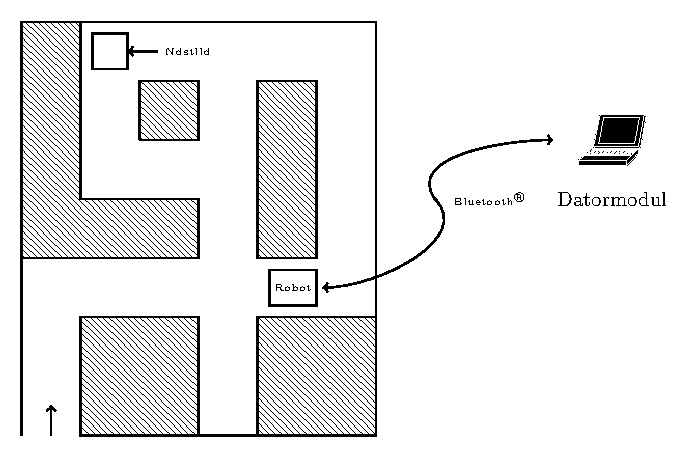
\includegraphics{images/overview}}
	\caption{Roboten i en labyrint \label{scene}}	
\end{figure}

I figur \ref{scene} befinner sig roboten i en exempelbana där den testats. För att konstruera roboten har hårdvaran inklusive till exempel sensorer och mikroprocessorer tillhandahållits av beställare, likväl som den nödvändiga programvaran för att ta fram mjukvara.

Detta dokument beskriver projektets genomförande och dess resultat. Bifogat finns de dokument som tagits fram under projektets gång, bland annat en projektplan och en teknisk beskrivning.

\pagebreak

\section{Problemformulering}
\textit{Redogör kort för kravbilden och referera till projektdirektiv och kravspecifikation för att läsa detaljer.}
\textit{Lägg återigen mest fokus på det som ni ansåg utmanande/intressant.}

För att klara uppgiften behövde roboten uppfylla ett antal grundläggande krav. Förutom att navigera i grottsystemet och identifiera den nödställde måste den även bestämma kortaste väg mellan ingången och den nödställde. För att kunna göra det delades grottsystemet in i moduler om 40x40 cm som var och en har ett unikt index, baserat på dess x- och y-koordinat. Även att rita upp en karta som representerar grottsystemets utformning var ett grundkrav. Nedan följer beskrivning av de övergripande utmaningarna som initialt identifierades. För en fullständig lista över kraven se appendix \ref{Kravspecifikation}.

\subsection{Tillräckligt bra sensorvärden}
För att roboten skulle ha en uppfattning om sin omgivning behövdes sensorerna. Dessa behövde sedan läsas av tillräckligt ofta och översättas med tillräcklig precision för att de skulle göra nytta i regleringen. 

\subsection{Kartläggning}
Kartläggningens utmaning var tvådelad. Den ena delen handlade om att hålla reda på hur roboten är orienterad samt vilken position den har. För att uppdatera rätt värden behövde roboten själv hålla koll på vilket värderstreck den var riktad i och vilken position den tagit sig till. Den andra, och mer komplexa, delen var utmaningen att komma fram till en struktur som gjorde uppdraget genomförbart. Information behövde lagras på ett sätt så att det gick att navigera i labyrinten på ett smidigt sätt och att beräkningen kunde ske effektivt.

\subsection{Kommunikation}
För att kunna överföra information mellan de olika modulerna var det viktigt att ha ett pålitligt kommunikationssystem. Utmaningen här låg i att den var essentiell för det framtida uvecklandet eftersom det inte gick att testa modulerna tillsammans annars. Därför var det viktigt att få denna del att fungera i ett tidigt skede.

\subsection{Integration av moduler}

Trots att arbetet delats upp i olika moduler var det viktigt att ha i åtanke att dessa skulle vara en del av ett större system. Även om modulerna kunde fungera felfritt var och en för sig fanns det en möjlighet att de skulle motverka varandra vid integrering av dem. Ett identifierat problemområde var att en moduls avbrott skulle kunna ta upp för mycket tid, vilket skulle medföra att de andra modulerna tappade effektivitet. 


\pagebreak

\section{Kunskapsbas}
\textit{Beskriv kortfattat och referera litteratur, datablad och dokumentation som ni använt er av för att genomföra projektet.}

Komponenterna som har använts under projektet finns nästan uteslutande beskrivna i datablad på kurshemsidans portal för datablad Vanheden\ref{hemsidan}. Där finns datablad för alla använda sensorer och för mikroprocessorn \verb+ATmega1284p+ som används av alla robotens moduler.

Tack vare tidigare lästa kurser fanns en god kunskapsbas hos projektmedlemmarna vid projektets start. I de fall då nödvändig kunskap saknades utibildade medlemmarna sig på egen hand inom det aktuella området. Detta gällde främst programmering i C, som ingen i projektgruppen tidigare hade arbetat med. 

De dokument som skrevs innan det praktiska arbetet påbörjades utgjorde också en viktig del och underlättade arbetet betydligt. Det dokument som användes mest var designspecifikaitonen, se appendix \ref{designspecifikation}, som i sin tur byggde på de tre förstudierna som genomfördes före projektets start. Förstudierna finns att läsa i appendix \ref{förstudier}

Till förfogande hade projektgruppen även en teknisk handledare tillhandahållen av ISY, instutitionen för systemteknik på Linköpings Universitet. Handledaren kom väl till pass då hårdvara krånglade och då svårare problem behövde diskuteras.

\pagebreak

\section{Genomförande}
\textit{Beskriv hur projektet har bedrivits och referera bland annat till LIPS-modellen, systemskiss, projektplan och designspecifikation. Observera att designspecifikationen belyser arbetsprocessen och inte den slutliga produkten så om ni uppdaterat designspecifikationen löpande under projektet så kan ni infoga t ex den version som var aktuell vid BP3.}

I följande avsnitt beskrivs hur projektet genomförts i de tre olika faserna \textit{före}, \textit{under} och \textit{efter}.

\subsection{Fas: Före}
Projektet har bedrivits enligt projektmodellen \textit{LIPS}. (referens?) Ett projektdirektiv tilllhandahölls av projektets beställare och var utgångspunkt vid framtagandet av projektets krav. Kraven delades in i tre olika prioriteringsnivåer: krav av prioritet 1 som måste uppfyllas, krav av prioritet 2 som borde uppfyllas i mån av tid och krav av prioritet 3 som kan ses som utvecklingmöjligheter. Kravens prioritering bestämdes utifrån projektdirektivet och projektgruppens intresseområden. 

Efter att kravspecifikationen färdigställts och godkänts av beställare påbörjades den förberedande fasen av projektet. En systemskiss upprättades där produktens övergripande funktionalitet och design beskrevs som ett första förslag på robotens utformning. En detaljerad beskrivning finns i appendix \ref{systemskiss}. 

Systemskissen låg sedan till grund för arbetet med projektplanen, där projektets aktiviteter togs fram. För att enklare kunna planera projektet identifierades alla aktiviteters föregångare för att tydligt kunna se vilka aktiviteter som behövde slutföras innan en annan kunde påbörjas. Lista över aktiviteter tillsammans med resten av projektplanen återfinns i appendix \ref{projektplan}. Där finns även tidplanen, vilken beskriver vilka aktiviteter som planerades att genomföras och hur dessa var beroende av varandra. Tidplanen uppdaterades kontinuerligt under projektets gång.

\subsection{Fas: Under}
Före projektets praktiska del starade gjordes, i par om två projektmedlemmar, förstudier inom områdena reglering, sensorer och kommunikation. Förstudierna låg sedan till grund för designspecifikationen som ger en ingående beskrivning av produkten. Syftet med designspecifikationen är att använda den som underlag vid det praktiska arbetet. Den skulle vara på den detaljnivå att all funktionalitet samt hård- och mjukvarudesign skulle vara tillräckligt utförligt beskriven för att kunna arbeta utefter dokumentet. Designspecifikationen i sin helhet hittas i appendix \ref{designspecifikation}. 

När designspecifikationen var färdigställt började det praktiska arbetet. Eftersom roboten hade tre tydligt förutbestämda delsystem föll det sig naturligt att det par som arbetat med respektive förstudie bar huvudansvar och jobbade mest med just det delsystemet hos roboten. Mjukvara för busskommunikation var något som tidigt färdigställdes eftersom arbetet med integreration av moduler skulle kunna påbörjas så tidigt som möjligt. Även avläsning av sensorer var också något som tidigt började arbetas med eftersom regleringen var beroende av att erhålla korrekta sensorvärden. För att mjukvaran skulle kunna testas i ett tidigt skede påbörjades även virning av hårdvara parallellt. 

Arbetet följde den ordning som listats i tidplanen för att på smidigaste sätt ta hänsyn till de beroenden som existerade mellan aktiviteter. Som nämnt uppdaterades tidplanen allt eftersom aktiviteter avklarades för att bättre visa det faktiska arbetets gång. Till hjälp vid utvecklingsarbetet av mjukvara till hårdvaran användes Atmel Studio. Mjukvaran till datorn utvecklades i Java. 

\subsection{Fas: Efter}
När det praktiska arbetet kommit till ett slut skrevs en teknisk dokumentation, se appendix \ref{TekniskDokumentation}. Denna redogör för hur roboten är konstruerad och vilka designbeslut som tagits. Användarhanledningen, se appendix \ref{Anvandarhandledning}, beskriver hur roboten ska användas.

Som avslut verifierades alla krav och produkten testades mot andra robotar som konstruerats med utgångspunkt från samma projektdirektiv

\pagebreak

\section{Teknisk beskrivning}
\textit{Redovisa det tekniska resultatet och förstudierna på ett lämpligt sätt. Detaljerade beskrivningar på grindnivå i hårdvaran eller på instruktionsnivå i mjukvaran är i detta sammanhang oftast ointressant. Referera den tekniska dokumentationen och förstudierna för beskrivning av detaljer. Lyft fram egna kreativa lösningar!}

Roboten består av fyra olika delsystem, moduler, som är designade för specifika ändamål monterade på ett chassi, se figur \ref{overview}. Huvudmodulen är det delsystem som sköter all kommunikation, både med dator via blåtand och mellan övriga moduler i form av I\textsuperscript{2}C-protokoll. Protokollet valdes utifrån resultatet i förstudien som inriktade sig på kommunikation, se appendix \ref{Kommunikation}. Huvudmodulen har även ansvar för att ta övergripande beslut speciellt om hur roboten ska utforska, alltså vilket håll roboten ska köra åt härnäst, enligt algoritmer beskrivna i förstudien som rör reglering, se appendix \ref{Reglering}. Huvudmodulen har slutligen också hand om intern kartläggning under tiden roboten utforskar och kommunicerar denna information till datormodulen vid tillfälle. 

\begin{figure}[!htbp]
\centering
\noindent\resizebox{.7\linewidth}{!}{
	
\documentclass[border=10px]{standalone}
\usepackage{tikz}
\usetikzlibrary{patterns}
\usetikzlibrary{shapes.arrows}
\usepackage{amssymb}
\usetikzlibrary{calc}
\usepackage{verbatim}
\usetikzlibrary{decorations.pathmorphing}

\begin{document}
	
\begin{tikzpicture}[scale=1,rotate=0]
		
	%Base
	\draw[thick, draw=black, fill=gray!10] (0,0) rectangle (6,10);

	%Wheels
	\draw[thick, pattern=north west lines, pattern color=black] (-.5,1) 		rectangle (0,2.5);
	\draw[thick, pattern=north west lines, pattern color=black] (-.5,7.5) 	rectangle (0,9);
	\draw[thick, pattern=north west lines, pattern color=black] (6,1) 		rectangle (6.5,2.5);
	\draw[thick, pattern=north west lines, pattern color=black] (6,7.5) 		rectangle (6.5,9);
	
	%Sensors
	\draw[thick, draw=black, fill=white]		(-.25,.25) 		rectangle 	(.5,.75);
	\draw[thick, draw=black, fill=white] 	(-.25,9.25) 		rectangle 	(.5,9.75);
	\draw[thick, draw=black, fill=white] 	(5.5,.25) 		rectangle 	(6.25,.75);
	\draw[thick, draw=black, fill=white] 	(5.5,9.25) 		rectangle 	(6.25,9.75);
	\draw[thick, draw=black, fill=white] 	(1.5,10.25) 		rectangle 	(4.5,9.5);
	\draw[thick, draw=black]				 	(2.5,9.5)			--		  	(2.5,10.25);
	\draw[thick, draw=black]					(3.5,9.5) --++ (0,.75);
	
	%Gripklo
	\draw[thick, draw=black, <-] (3,10.25) --++ (0,.72) node[above] {Gripklo};
	
	%Lidar lite
	\draw[thick, draw=black, <-] 			(1.5,10.25)  		--+ 		  	(135:1) node[above, align=center] {\verb+LIDAR-Lite v2+ \\ med servo};
	%Identifierare av nödställd
	\draw[thick, draw=black, <-]				(4.5,10.25)		--+			(45:1)  node[above] {\verb+IRM-8601-S+};
	
	%IR sensorer
	\draw[thick, draw=black, <-]				(-.25, 9.75) 	--+			(135:1) node[above] {\verb+GP2D120+};
	\draw[thick, draw=black, <-]				(-.25, .25) 		--+			(225:1) node[below] {\verb+GP2D120+};
	\draw[thick, draw=black, <-]				(6.25, 9.75) 	--+			(45:1) node[above] {\verb+GP2D120+};
	\draw[thick, draw=black, <-]				(6.25, .25) 		--+			(315:1) node[below] {\verb+GP2D120+};
	
	\draw[thick, draw=black, fill=white]					(2.5,4.5)		rectangle	(3.5,5.5);
	
	%Gyro
	\draw[thick, draw=black, <-] (3.5,5) --++ (.25,0) node[rotate=270, above] {\verb+MLX90609+};
	
	%Arrows and text
	%\draw[thick, ->]  (3,11) node[left, align=center] {\verb+LIDAR-Lite v2+ \\ + detektor av nödställd} -- (3,10.25);
	%\draw[thick, <->] (0.5,0.5)  --  (5.5,0.5) node[left=-14pt,midway, fill=gray!10] {\verb+GP2D120+};
	%\draw[thick, <->] (0.5,9.5) -- (3,9) node[right=-14pt,fill=gray!10] {\verb+GP2D120+} -- (5.5,9.5);
	%\draw[thick, ->] (4.5,5) node[above] {\verb+MPU-6500+} -- (3.5,5);
	
	%Sensormodul
	\node (sensormodul) at (3,6.75) [thick, draw=black, minimum width=3cm, minimum height=1.5cm, align=center, fill=white] {Sensormodul \\ \verb+ATmega1284p+};
	
	%Huvudmodul
	\node (huvudmodul) at (3,3.25) [thick, draw=black, minimum width=3cm, minimum height=1.5cm, align=center, fill=white] {Huvudmodul \\ \verb+ATmega1284p+};
	
	%Styrmodul
	\node (styrmodul) at (3,1.25) [thick, draw=black, minimum width=3cm, minimum height=1.5cm, align=center, fill=white] {Styrmodul \\ \verb+ATmega1284p+};
	
	%I2C-buss
	\draw[thick, draw=teal] ($(sensormodul.north east) + (.25,0)$) -- ($(styrmodul.south east) + (.25,0)$);
	\draw[thick, draw=teal] ($(sensormodul.north east) + (.5,0)$) -- ($(styrmodul.south east) + (.5,0)$);
	\node (i2c) at ($(sensormodul.north east) + (0.375,.25)$) [text=teal] {\small I\textsuperscript{2}C};
	
	\draw[thick, draw=teal, fill=teal] ($(sensormodul.south east) + (0,.25)$) --+ (.25,0) circle [radius=.05cm];
	\draw[thick, draw=teal, fill=teal] ($(sensormodul.south east) + (0,.5)$) --+ (.5,0) circle [radius=.05cm];
	
	\draw[thick, draw=teal, fill=teal] ($(huvudmodul.south east) + (0,.25)$) --+ (.25,0) circle [radius=.05cm];
	\draw[thick, draw=teal, fill=teal] ($(huvudmodul.south east) + (0,.5)$) --+ (.5,0) circle [radius=.05cm];
	
	\draw[thick, draw=teal, fill=teal] ($(styrmodul.south east) + (0,.25)$) --+ (.25,0) circle [radius=.05cm];
	\draw[thick, draw=teal, fill=teal] ($(styrmodul.south east) + (0,.5)$) --+ (.5,0) circle [radius=.05cm];
	
	%Koppling till sensormodul
	\draw[thick, draw=violet] (.5,9.5) --++ (.25,0) --++ (0,-2.5) --++ (0.75,0) ;
	\draw[thick, draw=violet] (.5,.5) --++ (.25,0) --++ (0,6.25) --++ (0.75,0);
	
	\draw[thick, draw=violet] (5.5,9.5) --++ (-.25,0) --++ (0,-2.5) --++ (-0.75,0);
	\draw[thick, draw=violet] (5.5,.5) --++ (-.25,0) --++ (0,6.25) --++ (-0.75,0);
	
	\draw[thick, draw=violet] (2,9.5) --++ (0,-2);
	\draw[thick, draw=violet] (4,9.5) --++ (0,-2);
	
	\draw[thick, draw=violet] (sensormodul.south) --++ (0,-.5);
	
	%Kopplingar till styrmodul
	\draw[thick, draw=olive] (styrmodul.east) --++ (1.5,0);
	\draw[thick, draw=olive] (styrmodul.west) --++ (-1.5,0);
	\draw[thick, draw=olive] ($(styrmodul.east) + (0,.25)$) --++ (1,0) --++ (0,6.25) --++ (.5,0);
	\draw[thick, draw=olive] ($(styrmodul.west) + (0,.25)$) --++ (-1,0) --++ (0,6.25) --++ (-.5,0);
	\draw[thick, draw=olive] (3,9.5) --++ (0,-1.75) --++ (-1.75,0) --++ (0,-6) --++ (.25,0);
	
	%Bluetooth
	\draw[thick, draw=black] (huvudmodul.east) --++ (2,0) node[right,minimum width=.75cm, minimum height=1cm, draw=black] (bt) {
\includegraphics{bluetooth}};
	
	\node (bt2) at ($(bt) + (2,0)$) [thick, draw=black, minimum width=.75cm, minimum height=1cm] {
\includegraphics{bluetooth}};
	
	\draw[thick, ->,line join=round,decorate, decoration={
    												snake,
    												segment length=5,
    												amplitude=1,
    												post=lineto,
    												post length=1pt}] 
    		($(bt.east) + (5pt,5pt)$) -- ($(bt2.west) + (-5pt,5pt)$);
    		
    \draw[thick, ->,line join=round,decorate, decoration={
    												snake,
    												segment length=5,
    												amplitude=1,
    												post=lineto,
    												post length=1pt}] 
    		 ($(bt2.west) + (-5pt,-5pt)$) -- ($(bt.east) + (5pt,-5pt)$);
    		 
    \draw[thick, draw=black] (bt2.east) --++ (.5,0) node[right, minimum width=3cm, minimum height=1.5cm, draw=black, fill=white] {Datormodul};
    
    \draw[thick, draw=black] ($(sensormodul.south west) + (.25,0)$) --++ (0,-2) node[midway, above, sloped] {\small avbrott};
    
    \draw[thick, draw=black] ($(styrmodul.north west) + (.25,0)$) -- ($(huvudmodul.south west) + (.25,0)$) node[right, midway] {\small avbrott};
	
	\end{tikzpicture}
	
\end{document}  
}
	\caption{Det totala systemet \label{overview}}	
\end{figure}

Sensormodulen är det delsystem som läser av sensorer och bearbetar informationen från dessa för att kunna utnyttja den vid styrbeslut. Den tar inga egna beslut utifrån informationen. Sensorerna är valda utifrån förstudien i appendix \ref{Sensorer}. Delsytem tre är styrmodulen som utför alla reglerberäkningar. För att kunna reglera rakt i korridor och svänga utifrån sensorvärden den fått in används en PD-regulator i enlighet med resultatet i förstudien i appendix \ref{Reglering}. Styrbeslut får den levererat från huvudmodulen. Den har även en LCD-display där utvalda data visas under körning. Datormodulen kan kommunicera styrkommandon till roboten men får främst information om karta och sensordata som den visar på skärmen. 

För att lösa problemet med att fästa sensorerna på roboten designades fästen som sedan skrevs ut med en 3D-skrivare. Detta gjorde att sensorerna enkelt och snyggt kunde fästas på roboten. Ett annat problem var att vid höga hastigheter gav hjulen på chassit inte tillräckligt hög friktion mot golvet och gled en del. För att öka friktionen knöts ballonger runt hjulen.

Utförligare teknisk beskrivning finns att läsa i appendix \ref{TekniskDokumentation}. 

BILD?

\pagebreak

\section{Resultat}
\textit{Beskriv kortfattat hur produkten används, hänvisa till användarmanualen.}
\textit{Beskriv vilken prestanda produkten har och hur det har testats, hänvisa till eventuella testprotokoll.}
\textit{Kommentera om produkten klarade de kraven som ställdes upp i kravspecifikationen. }

I detta avsnitt beskrivs resultatet av projektet.
\subsection{Beskrivning av produkten}
Roboten har olika körningar den kan genomföra. Dessa är söka av labyrint och köra kortaste väg och lämna förnödenhet efter att labyrinten är utforskad. Vilken körning den ska göra ställs in med knapptryck på en knapp monterad på roboten. 

Roboten kan både köra autonomt och styras manuellt från dator. I manuellt läge kan styrkommandon skickas genom att använda piltangenterna. Manuellt kan även körningar i autonomt läge startas istället för att trycka på den monterade knappen. 

På dator går utvalda sensorvärden att se i grafer och robotens utforskade del av labyrinten går att se när roboten kör autonomt.

Mer om hur roboten kan användas och felsökas finns att läsa i appendix \ref{}

\subsection{Robotens prestanda}
Roboten kan ta sig fram med en hastighet av i storleksordningen 1 m/s. Detta är \textcolor{red}{60 }\% av maxhastigheten. Vid sväng används en hastighet \textcolor{red}{70 }\% av maxhastigheten för svängar på 90 respektive 180 grader. Regleringen vid körning är inte beroende av att korridorerna är exakt raka utan roboten kan hålla sig ifrån väggen ändå. Sensordata processas och skickas i en sådan takt så att reglering sker felfritt. Robotens beslutsfattande sker så snabbt att det inte märks med blotta ögat utan det ser ut som att den endast kör på. 

\subsection{Test}
Testning av robotens funktionalitet skedde i olika steg. För att testa I\textsuperscript{2}C-kommunikationen användes först en färdigprogrammerad I/O-enhet tillsammans med huvudmodulens processor. När den verkade fungera användes en annan processor för att testa ytterligare implementationer.  Parallellt med detta konfigurerades sensorerna så att de skulle ge ut korrekta sensorvärden. Först när detta var klart testades regleringen. När regleringen fungerade påbörjades bantester för att testa avsökningsalgoritmen. För protokoll över bantester se \ref{}. 

Alla de krav med prioritet 1 som initialt ställdes upp i kravspecifikationen har uppfyllts. Inga prioritet 2 krav har implementerats.

\pagebreak

\section{Slutsatser}
\textit{Slutsatser
Sammanfatta arbetet. 
Lyft fram det ni är mest nöjda med.
Reflektera över resultatet såväl tekniskt som över genomförandet. Referera efterstudien.}
\textit{Framtida arbete
Vad skulle ni göra annorlunda om ni skulle göra om samma uppdrag?
Vad skulle ni vilja utveckla om ni fick mer tid?
Hur skulle ni tänka er att ändra uppgiften för att göra den ännu mer intressant?}

I detta avsnitt presenteras projektets slutsatser samt dess framtida utvecklingsmöjligheter.

\subsection{Slutsatser}

Gruppen har arbetat effektivt från start. Arbetet med dokumenten i början speciellt designspecifikation och projektplan har varit till god hjälp som underlag för det praktiska arbetet. Hade mindre tid lagts på dessa dokument hade kanske inte projektet gått så smidigt som det gjort från start. Det praktiska arbetet har med parindelning och realtivt jämn arbetsfördelning flutit på utan några större problem på gruppnivå. Om problem uppstått har gruppen tillsammans försökt lösa dem. Modulindelningen har inte hindrat arbetet i stor utsträckning då resterande gruppmedlemmar kunde skriva dokumenattion och kod vid tillfällen då roboten var upptagen.
Mest nöjda förslag : 
\begin{itemize}
\item Arbetsmässigt : Gruppen har samarbetat bra och tagit ansvar vilket har gjort att arbetet flutit på väldigt bra och aktiviteter har blivit gjorda i tid. 
\item Produktmässigt: Roboten snabb. Avsökningsalgoritmen fungerade från början vid testning. IR-sensorer bra
\end{itemize}

En utvärdering av projektets delar och stösta problem går att läsa i appendix \ref{}

\subsection{Att tänka på till nästa gång}

Hade projektet genomförts igen hade en del saker kunnat göras annorlunda. En längre tanke om aktiviteterna i projektplanen hade varit en sak att fokusera på för då hade det kanske insetts att vissa aktiviteter gick in i varandra och på så sätt hade dessa kunnat formuleras om. En annan sak är att från start använda ett pålitligare sätt att mäta avlagd sträcka än lasersensorn, alltså från början göra mer omfattande undersökningar om alternativ av sensorer. En tredje sak hade varit att försäkra sig om att det fölr varje modul finns två personer som är insatta i hur varje del av koden fungerar för att minska beroendet av en viss person. I detta projekt har situationen inte skapat några problem utan enbart utgjort en risk. Den fjärde och sista punkten hade varit att från början sätta upp standard för testprotokoll och dokumenterat hur diverse problem lösts. Detta för att inte samma sak felsöks flera gånger när en lösning funnits tidigare. 

\subsection{Utvecklingsmöjligheter}
Hade gruppen haft mer tid till förfogande, eller om någon vill ta vid där detta projekt avslutas, finns det några funktioner med utvecklingsmöjligheter. Ett mindre prioriterat krav, som i genomfört projekt inte har uppfyllts, är att roboten ska klara av att navigera i öppna rum. Det är något som är relevant för en undsättningsrobot eftersom grottsystem sällan består av enbart korridorer. En annan kvalitet som skulle höja robotens förmåga som undsättare är att roboten skulle klara av att genomföra svängar som kan vara av godtycklig vinkel, inte bara 90 och 180 grader. 

En annan utvecklingsmöjlighet är att förbättra datorprogrammet och göra det snyggare grafiskt. Ju mer användarvänligt och visuellt attraktivt programmet är, desto roligare är det för en användare att använda produkten. En bättre optimerad avsökning kan även vara värd att arbeta på.

\subsection{Utveckla uppgiften}
En utvecklingsmöjlighet med uppgiften, som inte nödvändigtvis försvårar den, kunde vara att istället för att en nödställd ska identifieras utöka antalet nödställda. Ytterligare en rolig grej hade varit om inte alla delar av labyrinten var på samma nivå, alltså att den skulle ha två våningar. 

\pagebreak

\section{Referenser}
\textit{Ange de referenser som hänvisas till från kappan. Nämn gärna också att fler referenser finns i bilagorna.}

\pagebreak
\addcontentsline{toc}{section}{Referenser}
%\bibliographystyle{ieeetr}
%\bibliography{references}

\pagebreak


\appendix

\end{flushleft}

\end{document}


